% LaTeX source for ``Complexity and Computation''
% Copyright (c)  2011  Allen B. Downey.

% Permission is granted to copy, distribute, transmit and adapt
% this work under a Creative Commons
% Attribution-NonCommercial-ShareAlike 3.0 Unported License:
% http://creativecommons.org/licenses/by-nc-sa/3.0/

% If you are interested in distributing a commercial version of this
% work, please contact Allen B. Downey.

% The LaTeX source for this book is available from
% http://greenteapress.com/complexity
% http://code.google.com/p/complexity

% This book was typeset using LaTeX .  The illustrations were
% drawn in xfig.  All of these are free, open-source programs.

%%----------------------------------------------------------------

% How to compile this document:
% If your environment provides latex, makeindex, and dvips,
% the following commands should produce a Postscript version
% of the book.

%        latex book
%        makeindex book
%        latex book
%        dvips -o book.ps book

% You will also need the following (fairly standard) latex
% packages: url, epsfig, makeidx, fancyhdr

% This distribution also includes a Makefile that should
% compile both the Postscript and PDF versions of the book.

%%-----------------------------------------------------------------

\documentclass[10pt]{book}
%\pdfminorversion=5
%\pdfobjcompresslevel=2

\usepackage[width=5.5in,height=8.0in,
  hmarginratio=3:2,vmarginratio=1:1]{geometry}

\usepackage[T1]{fontenc}
\usepackage{textcomp}
\usepackage{mathpazo}

\usepackage{url}
\usepackage{fancyhdr}
\usepackage{graphicx}
\usepackage{amsmath, amsthm, amssymb}
\usepackage{exercise}
\usepackage{makeidx}
\usepackage{setspace}
\usepackage{hevea}
\usepackage{verbatim}
\usepackage{upquote}
\usepackage{parskip}

\newcommand{\thetitle}{Think Complexity}
\newcommand{\theversion}{1.2.2}

\title{\thetitle}
\author{Allen B. Downey}

% these styles get translated in CSS for the HTML version
\newstyle{a:link}{color:purple;}
\newstyle{p+p}{margin-top:1em;margin-bottom:1em}
\newstyle{img}{border:0px}


\makeindex

\newtheorem{exercise}{Exercise}[chapter]

\begin{document}


\setcounter{chapter}{14}
\chapter{Case study: Zipf's Law and Music}

{\em Max Ward (20748588)}

\section{Music as Language}

Zipf's law was introduced in Chapter 5. To recapitulate, it posits that the frequency of a word is inversely proportional to its rank. The rank of a word being defined as its index in a frequency table. The canonical example is that of the words in a long piece of literature, usually a novel. If we rank each word by how often it appears, we should see a specific relationship between a word's frequency, and its rank. Zipf's law is a classical example of a scale-free distribution, and is defined by $f = r^{-a}$ where $f$ is frequency and $r$ is rank. A frequency distribution is said to be Zipfian if $a \approx 1$. Because of this, when plotted on a log-log scale (equivalent to taking the log of both sides), a Zipfian distribution appears to be a line with slope $m \approx -1$. Though Zipf's law is typically described in terms of novels, and thus written language, it actually refers to any natural language. Natural language is generally regarded to be any non-contrived language---which is to say that its use and invention is unpremeditated. Clearly most written and spoken languages are natural languages, however, music is also a type of natural language.

Music, among other art forms, is regarded as a form of communication. Like other forms of human communication, it has structure and rules. While I shall not give a formal definition of these, the reader may refer to \url{http://en.wikipedia.org/wiki/Music_theory} for a concise overview. This chapter investigates Zipf's law in music. This was done by using the MIDI file type, which is a relatively simple and widely used way to encode digital music.


\begin{exercise}

There are specific parts of the human brain involved in language. For example, damage to Broca's area can profoundly affect one's ability to understand spoken and written language. Does an analogous region exist for processing music? (Hint: try searching for `Amusia'.)

\end{exercise}

\section{The MIDI Format}

The MIDI file format comprises a header and a series of one or more tracks. Every MIDI track also contains a header, which is followed by a sequence of events. There are many MIDI event types. However, the only two which we consider in this investigation are the `Note On' and `Note Off' events. A Note On event has a time, a velocity, and a note code. The time represents when it is to be played, the velocity is the force with which it is to be played, and the note code refers to the sound being played. It should be noted that velocity is not volume. It is possible than a MIDI instrument could have a linear velocity-volume relationship, but it could be exponential, logarithmic, or anything else. There are 128 distinct note codes in the MIDI format. These are analogous to an extended piano (which has 88 keys), with each increment indicating a semitone increase in sound frequency.

\begin{figure}
	\centering
  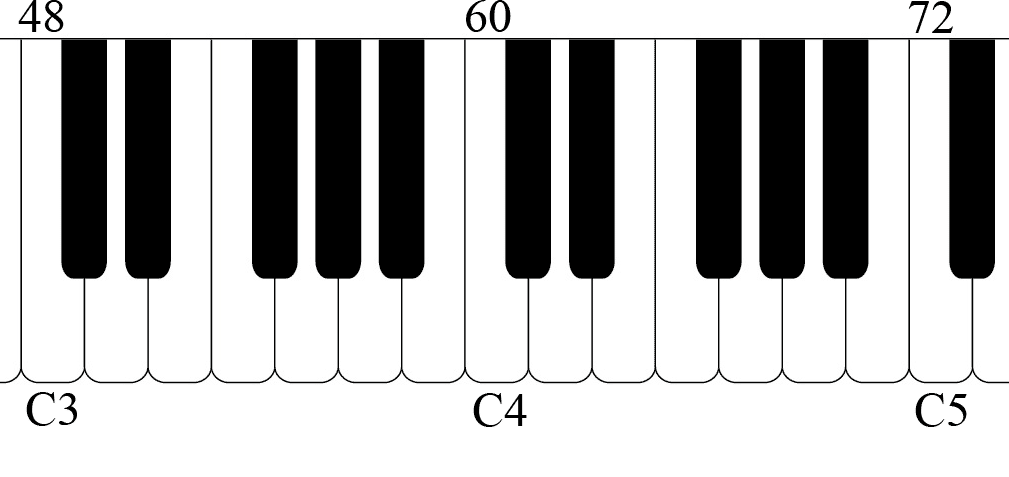
\includegraphics[scale=0.3]{Keyslol}
  \caption{The relationship between notes on a keyboard and MIDI codes. The bottom labels are notes, the top labels are MIDI codes}\label{fig:keys}
\end{figure}

Parsing the MIDI format can be difficult and, as such, it is often relegated to a library. Python does not come with an easy to install MIDI parsing library. However, an open source effort called \texttt{python-midi} is available on Github under the MIT licence. It can be found at \url{https://github.com/vishnubob/python-midi}. Download or clone the repository and use the source files in your project. Once they are in the same folder, you should be able to import them like any Python library. I have provided a basic example that loads a MIDI file, given a file name from the command line. The \texttt{fileio} module is part of \texttt{python-midi}. It contains functions related to reading and parsing MIDI files.


\begin{verbatim}
import sys
import fileio

def main(name, fname, *args):
    pattern = fileio.read_midifile(fname)
    print pattern

if __name__ == '__main__':
    main(*sys.argv)

\end{verbatim}


The way MIDI patterns are represented in \texttt{python-midi} is straightforward. A pattern is a list of tracks. A track is a list of events. Every event has a type, and associated meta-data. All of these classes also have the \texttt{\_\_repr\_\_} method overloaded. This makes it easy to determine what information is available. A quirk of some older MIDI files is that a Note On event with velocity 0 is equivalent to the corresponding Note Off event. Keep this in mind when experimenting with MIDI files.

The Classical Archive has some excellent MIDI encodings of classical music (available at \url{http://www.classicalarchives.com/midi.html}). You may also wish to find some songs from other sources. Many people have made their MIDI versions of songs freely available on the Internet. There is also software that allows the user to write MIDI music using a graphical environment. If you are so inclined, it is possible to analyse your own compositions.


\begin{exercise}
Research the MIDI format. How hard do you think it would be to write your own parser? Remember, if you improve \texttt{python-midi}, submit a pull request to Github.
\end{exercise}

\begin{exercise}
Attempt to write a script that outputs the number of distinct notes in a MIDI file. My solution is available at URL.
\end{exercise}


\section{Words and Music}

Zipf's law refers to the frequency of words found in a large corpus of natural language. It is hard to see how the concept of a word could apply to musical compositions. Of course, any interpretation of a word in music is necessarily arbitrary and somewhat open to interpretation. Despite this, I shall now describe several feasible candidates. The most obviously irreducible component of a musical composition is the note. Building upon this starting point, one might analyse the velocities, lengths, or the spacing between similar notes. More complex interpretations may attempt to group notes into structures like chords or melodies. I shall, however, start with a much simpler interpretation.

\subsection{Notes}
\label{sec:note_group}
As I have said, a piece of music can be broken up into notes. If we define a word as a single note, we can then collect the frequencies of these notes, and thence subject them to Zipfian analysis. This necessitates going through every MIDI event in every MIDI track for any given pattern. The \texttt{python-midi} package makes this quite easy, as tracks and events are represented as objects that inherit from \texttt{list}. Here is a simple function that returns all the notes (in no particular order) given the path to a MIDI file.

\begin{verbatim}
def get_notes(fname):
    pattern = fileio.read_midifile(fname)
    notes = []
    for track in pattern:
        for event in track:
            if event.name == "Note On" and event.data[1] > 0:
                notes.append(event.data[0])
    return notes
\end{verbatim}

The first line reads and parses the MIDI into a pattern. The following two loops examine every event in the pattern. Every time a genuine Note On event is spotted (remember that a Note On event with velocity 0 is actually a Note Off event) it is added to the \texttt{notes} list. It should be pointed out that meta data associated with an event is stored in \texttt{event.data}. For Note On events, index zero is the MIDI note, and index one is the velocity. After executing this function, we now have everything we need to calculate frequency as a function of rank.


\subsection{Consecutive Notes}
A more versatile way of using note frequencies is to consider sequences of consecutive notes. This is achieved by sorting all the notes in the MIDI file by order of appearance, then running a sliding window of fixed size over the notes. This results in a much larger corpus of possible words. For example, a window size of two will have $128^2$ possible words, every combination of two MIDI notes. Having a window size of one is the same as the approach described in Section \ref{sec:note_group}. Having too large a window size can be problematical, as it often results in having many words with very low frequency. I found that a window size of two was typically the best. Very long pieces of music may work with larger window sizes, however.

\begin{exercise}
Implement the sliding window note analysis technique. Note On objects have a member called \texttt{tick}, which is the number of ticks before they appear in the MIDI song. This can be used for sorting. My solution can be found at \url{thinkcomplex.com/SlidingWindow.py}.
\end{exercise}


\subsection{Note and Velocity Pairs}
I have outlined how we could use the occurrences of notes as an interpretation of words. However, a Note On event has two components; the note and its velocity. Another reasonable interpretation of a word is to use a tuple of these data. A quirk of the \texttt{python-midi} package is that \texttt{event.data} is actually a list. Because of this, I have used the built-in function \texttt{tuple} to convert it to a tuple in the code snippet presented below.

\begin{verbatim}
def get_notevelocities(fname):
    pattern = fileio.read_midifile(fname)
    notes = []
    for track in pattern:
        for event in track:
            if event.name == "Note On" and event.data[1] > 0:
                notes.append(tuple(event.data))
    return notes
\end{verbatim}


\begin{exercise}
Can you think of any problems with this method? Would using a sliding window over note and velocity pairs be a good idea?
\end{exercise}



\subsection{Note Intervals}
Thus far, all the word interpretations I have described deal with events directly. As an alternative, we may wish to take a more high level approach. For every MIDI note frequency that appears in a MIDI pattern, the intervals between specific notes could be recorded. For example, if the note code 60 appears at tick 110, then later at 120, then again at 135, we would record intervals of 10 and 15. Such intervals could be collected for every note in the MIDI pattern, and collated into one list. We can then calculate the rank and frequency of note intervals for further analysis.

\begin{exercise}
Implement the \texttt{get\_noteintervals} function. Modifying the \texttt{get\_notes} function might make this easier. Don't forget to sort all MIDI events by tick first. (Hint: use a dictionary to store the last occurrence of every note code.)
\end{exercise}

\begin{exercise}
Can you think of any other aspects of music that might reasonably conform to Zipf's law? If you can think of any, implement a getter function like those present in this section.
\end{exercise}




\section{Scale-free Music}
\label{sec:scalefreemusic}
In Chapter 5, we created a number of useful classes and functions for dealing  power law distributions. A copy of these files will be helpful in analysing the words described in the previous section. Using the \texttt{Pmf.py} and \texttt{Zipf.py} modules, a histogram can be created for ranks and frequencies. From here, we can plot a log-log graph of ranks versus frequency. If the graph looks somewhat like a straight line with slope $\approx -1$ then this confirms that a rank-frequency function is Zipfian. For analysis I chose `Wish You Were Here' and `Comfortably Numb' by Pink Floyd, Rachmaninov's `Allegro Ma Non Tanto' (No. 3 in D minor, Op. 30), and Brahms's `Hungarian Dance' No. 1. First, let us examine a simple distribution of single note frequencies.


\begin{figure}[!htb]
\minipage{0.4\textwidth}
  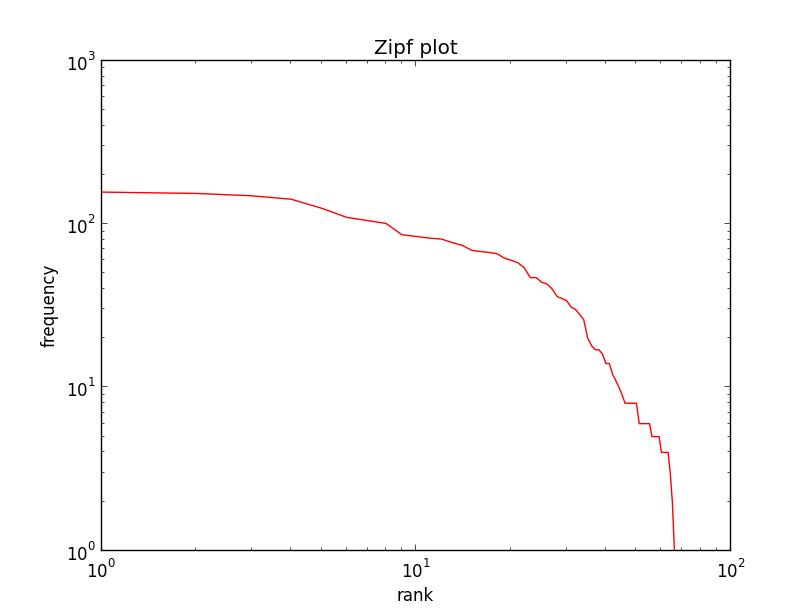
\includegraphics[width=\linewidth]{hungdan_notes_1}
  \caption{Hungarian Dance No. 1 using single notes}\label{fig:hungdan_notes_1}
\endminipage\hfill
\minipage{0.4\textwidth}
  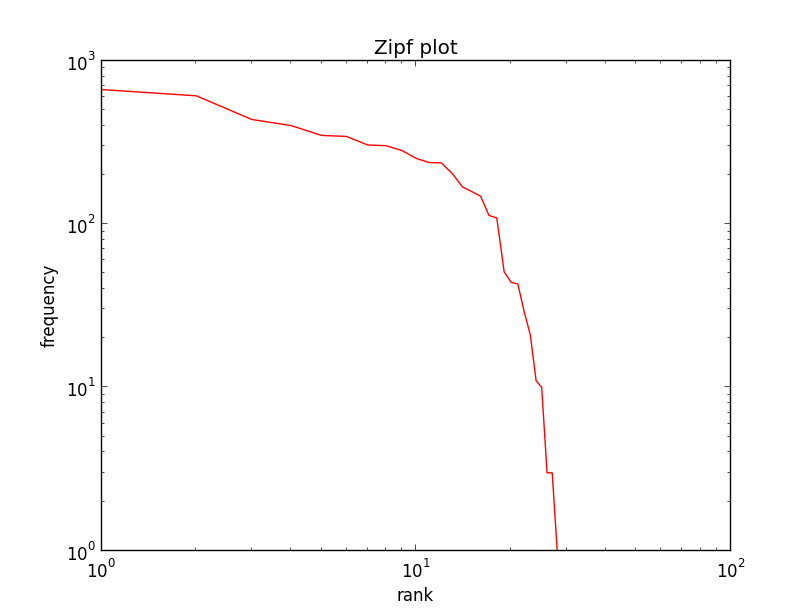
\includegraphics[width=\linewidth]{wish_notes_1}
  \caption{Wish You Were Here using single notes}\label{fig:wish_notes_1}
\endminipage\hfill
\minipage{0.4\textwidth}%
  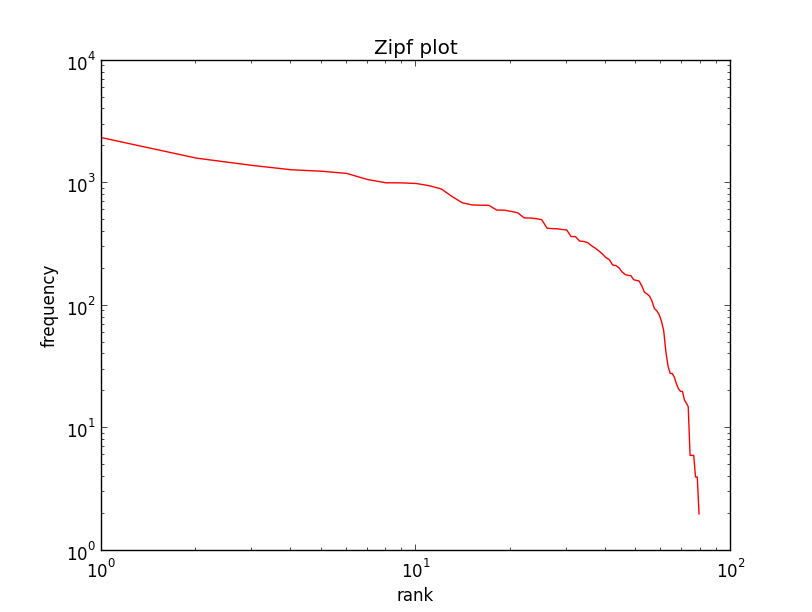
\includegraphics[width=\linewidth]{rach_notes_1}
  \caption{Allegro Ma Non Tanto using single notes}\label{fig:rach_notes_1}
\endminipage\hfill
\minipage{0.4\textwidth}%
  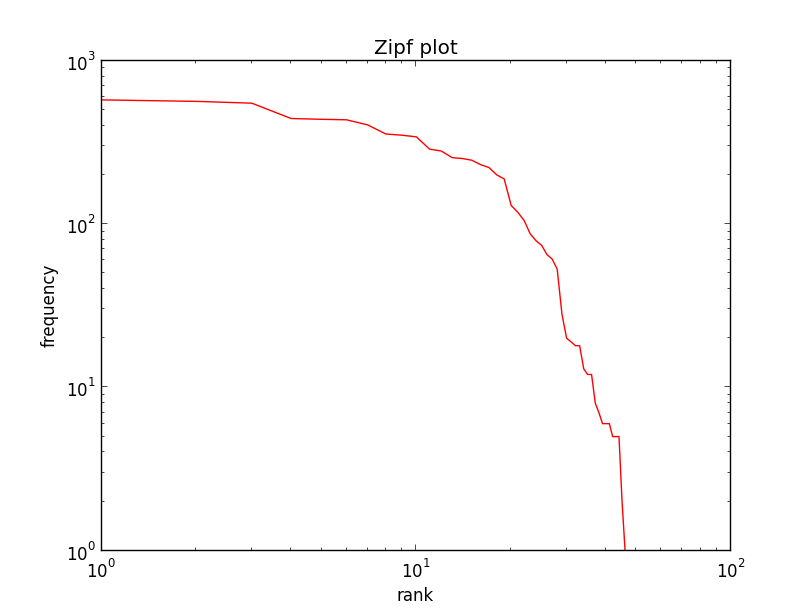
\includegraphics[width=\linewidth]{comf_notes_1}
  \caption{Comfortably Numb using single notes}\label{fig:comf_notes_1}
\endminipage
\end{figure}

Figures \ref{fig:hungdan_notes_1} - \ref{fig:comf_notes_1} show log-log plots of frequency versus rank for my selected songs. These graphs only look somewhat Zipfian. Typically a graph starts like a line, but drops off quickly towards the end. It is important to remember that songs are generally only a few minutes long, and are not comparable in size to a novel. As such, I argue that this constitutes evidence that music exhibits Zipf's law to a remarkable degree. To further test my hypothesis, I ran the  same test, except using a sliding window of size two. This means that every pair of adjacent notes was used as a `word' for the purposes of calculating frequency.



\begin{figure}[!htb]
\minipage{0.4\textwidth}
  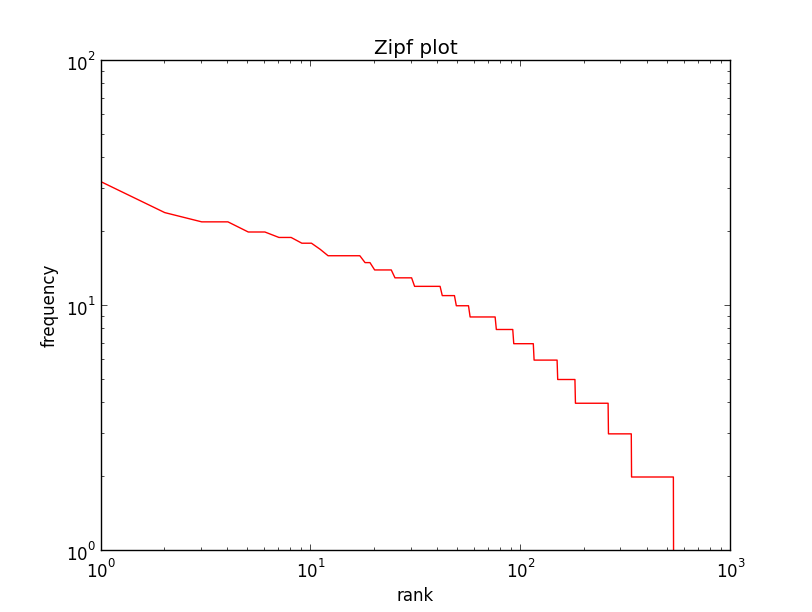
\includegraphics[width=\linewidth]{hungdan_notes_2}
  \caption{Hungarian Dance No. 1 using a sliding window over pairs of notes}\label{fig:hungdan_notes_2}
\endminipage\hfill
\minipage{0.4\textwidth}
  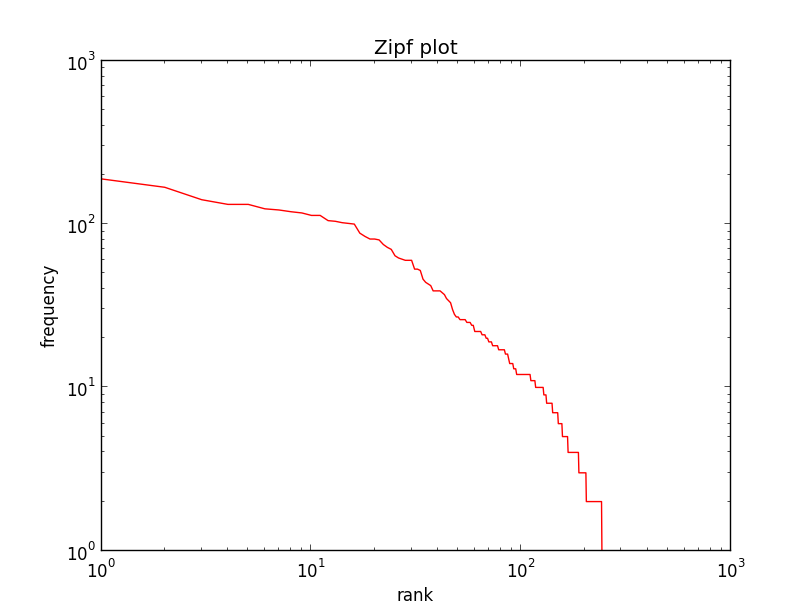
\includegraphics[width=\linewidth]{wish_notes_2}
  \caption{Wish You Were Here using a sliding window over pairs of notese}\label{fig:wish_notes_2}
\endminipage\hfill
\minipage{0.4\textwidth}%
  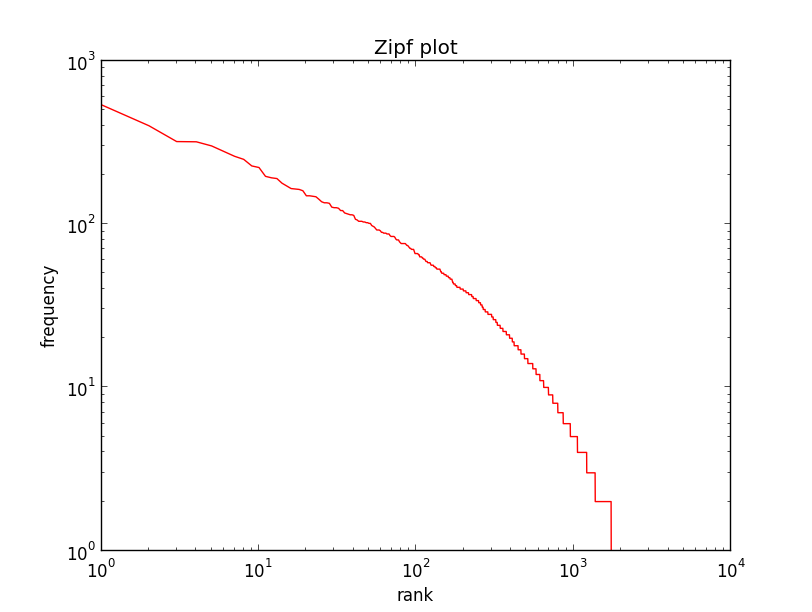
\includegraphics[width=\linewidth]{rach_notes_2}
  \caption{Allegro Ma Non Tanto using a sliding window over pairs of notes}\label{fig:rach_notes_2}
\endminipage\hfill
\minipage{0.4\textwidth}%
  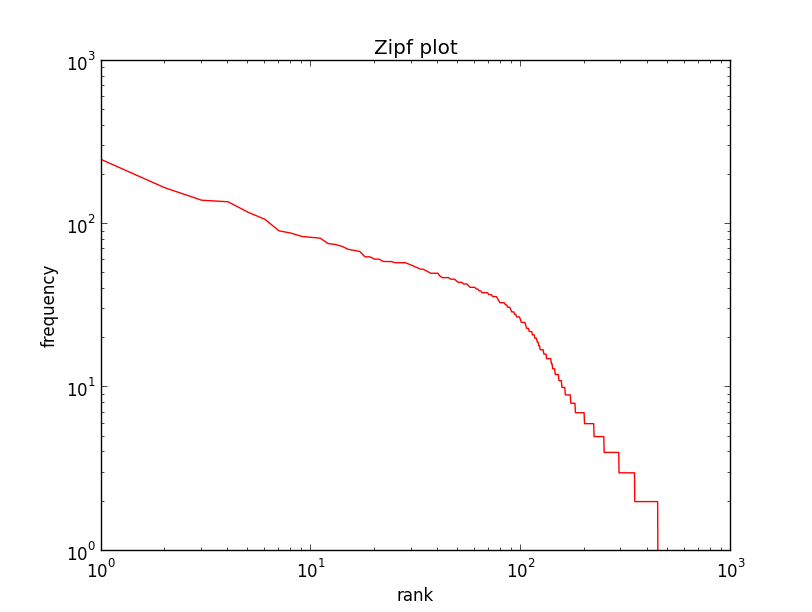
\includegraphics[width=\linewidth]{comf_notes_2}
  \caption{Comfortably Numb using a sliding window over pairs of notes}\label{fig:comf_notes_2}
\endminipage
\end{figure}

As can be seen in Figures \ref{fig:hungdan_notes_2} - \ref{fig:comf_notes_2}, using a sliding window over note pairs appears a little more compelling. A similar pattern emerges: a line that eventually drops off towards the end. However the suddenness of the drop off is typically less, and the extent of the line typically larger. Brahms's Hungarian Dance No. 1 in particular looks notably like the Zipf distributions analysed in Chapter 5.


\begin{exercise}
Use some music of your choosing to recreate these graphs. Do you see a similar pattern?
\end{exercise}

\begin{exercise}
In the previous chapter, several other interpretations of a musical `word' were discussed. Test if they follow Zipf's law in the MIDI tracks you chose.
\end{exercise}



\section{The Beauty of Context}

In 1955, Simon published a paper which attempted to explain Zipf's law. He noted that the law had been observed in many vastly different, and probably unconnected, domains. For example, Zipf's law can be found in the distribution of scientists and their published papers, and as we discovered in Chapter 5, in the rank of cities by population. A copy of Simon's original paper, "On a Class of Skew Distribution Functions", can be found here \url{http://www.uvm.edu/~pdodds/teaching/courses/2009-08UVM-300/docs/others/1955/simon1955.pdf}. It contains a lengthy, and somewhat impenetrable, explanation of why Zipf's law might exist. The essence of his idea is quite straightforward, however.

Simon posits that large bodies of literature are generally constructive. Consecutive words are appended one by one to the end, which is precisely what is happening as I write this. As words are added, a context is created. As this context emerges ex nihilo, it favours the reuse of previous words to maintain the context. In a similar sense, the introduction of new words is also inhibited. This model presupposes that context is an essential part of communication. Intuitively, it is easy to see the importance of context to human communication. Say that we take a novel and randomly shuffle sentences around. It is overwhelming likely that the book is now unintelligible. The linear construction of the book's context would have been destroyed. Similarly, take a piece of music and shuffle around movements randomly. Though each individual component would make sense, the cohesion of the whole would be destroyed.

As recently as 2005, Bill, Juan, and Penousal used Zipf's law to definite a fitness function for judging music. Such a function is useful for the computer generation of pleasant music, and this was their motivation. They used a large array of tests, encompassing and eclipsing those presented here. Much as we found in Section \ref{sec:scalefreemusic}, they discovered that Zipf's law was present in musical compositions. Furthermore, they found that it was not present in non-music compositions. In addition to this, they were able to train an artificial neural network to differentiate between genres of music, using the slope of the regression line for the log-log diagram of frequency and rank. It was also able to accurately distinguish the work of different composers within the same genre. On the strength of their findings, they concluded that Zipf's law was a necessary, though not complete, precondition for aesthetically pleasing music. The interested reader can find a copy of their paper, "Zipf's Law, Music Classification, and Aesthetics", at \url{http://www.idi.ntnu.no/emner/tdt04/2010%20articles/Zipf-music-johannes.pdf}.

Clearly, claiming that music and language are similar because they both exhibit Zipf's law is an argument from analogy, and thus is also an holistic argument. However, what about Simon's model? Does it appear to be reductionist, or holistic? Furthermore, is Simon's constructive argument based on an instrumentalist point of view, or realist? To clarify, we have two systems, that of language, and that of music. Both have the same property, Zipf's law. A holist would argue that this is because such a law is a fundamental or essential property of both. However, Simon has argued that this property can be explained constructively; at a very low level, music and language are similar, and as a result they share an emergent property. Sometimes the lines between holism, reductionism, instrumentalism, and realism can be ill-defined. This is a good example. Regardless, it is clear that Zipf's law is present in music. `Why' is another, and perhaps more intractable, question.

\begin{exercise}
Find examples of white noise, pink noise, and brown noise on the Internet. (YouTube is a good place to look.) Which do you prefer, and why? (Hint: Pink noise is also called $1/f$ noise.)
\end{exercise}

\begin{exercise}
Have a look at some of the properties that yielded a Zipfian distribution in Bill, Juan, and Penousal's paper. See if you can implement them, and reproduce their results.
\end{exercise}


\end{document}
